\chapter{Sequential Building Blocks}

In order to design complex systems, a suitable 
abstraction is required for building them.  This requirement stems from the
limitations of the human mind to only manage about a dozen items
at once.  A complex system containing hundreds of components
simply cannot be organized in one pass.  Instead, the components 
are organized into larger units which compose the system. Thus, 
the number of components need to be considered at a development stage is reduced
by an order of complexity. These intermediate units should have
a high utility and be modular.  In other words, they should be
useful and applicable in a wide variety of design situations.

As an example, consider the design problem of writing a technical 
document describing the operation of a pacemaker for a human heart.
This process does not begin by thinking about the spelling of
the individual words, instead it makes more sense to first
draft an outline.  This outline is an abstraction of the 
written document, it is a simplified representation of the final 
written document.  In somewhat the same way as an author ignores
spelling issues when constructing the outline, a designer is not concerned with 
the operation of AND and OR gates
when designing a digital-signal processing chip.  

Clearly, choosing components, or as they are called ``basic 
building blocks," which are reusable and have non-overlapping
functionality, result in a small number of highly useful 
components.  The set of available building blocks has largely 
been determined by the electronics industry which provides basic
blocks as off-the-shelf prepackaged components.  These 
time-tested components have established themselves over the years 
as the accepted language of hardware design. 
Several sequential logic building blocks are examined, next.  
The word ``sequential" in their name implies that these building 
blocks are different from those presented in Chapter 4 because 
they have memory. 

Like the combinational building blocks shown in 
Figure~\ref{fig:Asys} each of the sequential basic building 
blocks have control and data inputs, and status and
data outputs.  In addition, being sequential devices, most
also have an edge-sensitive clock input.  First to be examined is 
the most basic sequential basic building block, the register.

\section{The Register}
\index{register|(}
\label{page:reg}
\begin{tabular}{|l|p{3.5in}|} \hline
Nomenclature:  & N-bit register                           \\ \hline
Data Input:    & N-bits vector $D=d_{N-1} \ldots d_1 d_0$.          \\ \hline
Data Output:   & N-bit vector $Q=q_{N-1} \ldots q_1 q_0$    \\ \hline
Control:       & 1-bit $C$              \\ \hline
Status:        & none                                   \\ \hline
Others:		& 1-bit edge-sensitive clock.  1-bit asynchronous
		active low reset.			\\ \hline
Behavior:      & 
			\begin{tabular}{c|c|c|c||c||c}
			$reset$ & $clk$          & $C$ & $D$ & $Q^+$ & comment \\ \hline
			0     & x            & x & x & $0$   & reset   \\ \hline
			1     & 0,1,falling  & x & x & $Q$   & hold  \\ \hline
			1     & rising       & 0 & x & $Q$   &  hold \\ \hline
			1     & rising       & 1 & D & D     &  load \\
			\end{tabular} \\ \hline
\end{tabular}
\\ \\
An N-bit register is very much like a wide D flip flop.  It samples
its N data inputs, denoted $D$ on the rising edge of the clock input.
Depending on the control input, $C$, the register either holds its current 
value when $C=0$ or loads the new value when $C=1$.  The stored value 
of the register is asserted on its output, denoted $Q$. The columns 
in the register's state table are organized from left to right, from 
highest priority to lowest priority.   Holding the
asynchronous active low reset line to 0 causes the stored value
and the outputs to remain at 0 regardless of the value on any other
input; the reset input has priority over all other inputs.

A timing diagram for a 4-bit register is shown in Figure~\ref{fig:RegTime}.
The initial value of the register is arbitrarily set to $A_{16}=0001_2$.  
Since the value of $Q$ is represented using four bits, its value on the timing
diagram is shown as a wide trace.  This reflects the fact that $Q$ is 
composed of many bits.  At time=10, a positive edge of the clock arrives
with $C=1$, hence the register loads $D=5_{16}=0101_2$, as its new value.  
The fact that the $Q$ outputs changes slightly after time=10 is an 
acknowledgment that the circuit elements inside the register have 
propagation delay.  The goofy behavior of the $C$ input around time=20 has
no effect on the $Q$ outputs of the register because the clock is not rising.
The rising clock edge at time=30 does not change the stored value of the 
register because $C=0$, hence the register holds its stored value.  The change
in the $Q$ output at $time 50$ results from the rising clock edge and $C=1$.

\begin{figure}[ht]
\center{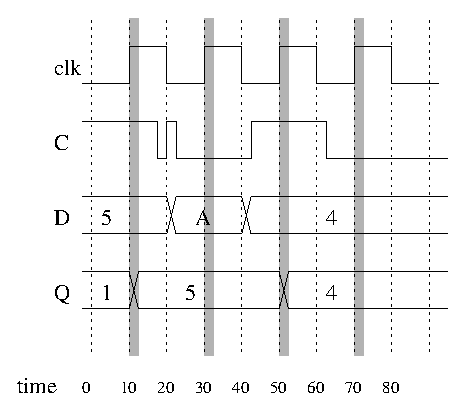
\includegraphics{./Fig6/RegTime}}
\caption{A timing diagram for a 4-bit register.}
\label{fig:RegTime}
\end{figure}
\index{timing!register}
\index{register|)}

An N-bit register is constructed using N, D flip flops.  A common error
committed by beginning students, and even some text books, is to AND the 
$clk$ and $C$ signals together, sending the AND gate output to the 
clock input of a D flip
flop.  This technique is incorrect because it causes the D flip flops to 
sample their input when the $clk = 1$ and $C$ rises, contrary to the behavior
described in the register's state table.  As a general rule, 
avoid modifying the clock signal unless it is absolutely necessary.

The correct construction of an N-bit register is shown in 
Figure~\ref{fig:reg}.   Two modes are present for this circuit, 
corresponding to $C=0$ and $C=1$.  When $C=1$, the four multiplexers 
shown in Figure~\ref{fig:reg}, all route the data input $D_i$ 
to the input of the D flip flop.  When a clock edge arrives,
each $D_i$ is loaded into its respective flip flop and
soon thereafter appears on the $Q$ output. 

\begin{figure}[ht]
\center{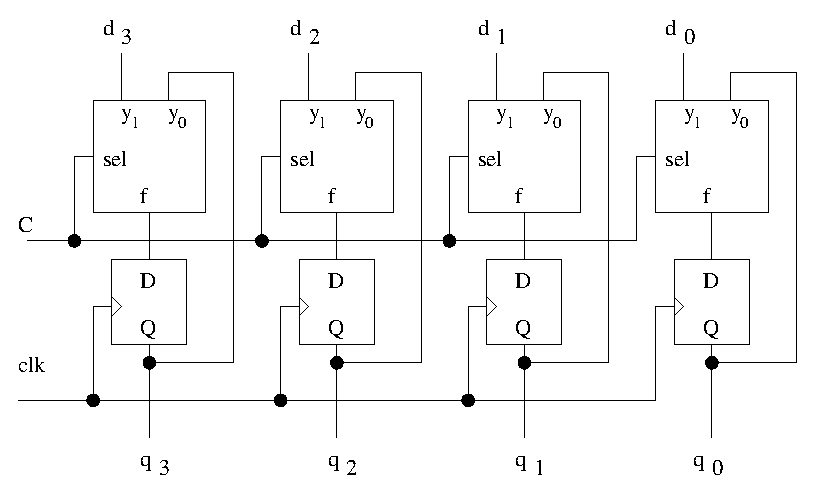
\includegraphics{./Fig6/reg}}
\caption{The internal organization of a 4-bit register.}
\label{fig:reg}
\end{figure}

When $C=0$, the four multiplexers shown in Figure~\ref{fig:reg}, 
all route their data output $Q_i$ back to the input of the 
D flip flop.  When a clock edge arrives, each $Q_i$ is  
loaded into its respective flip flop and soon thereafter appears 
on the $Q$ output. Thus, the $Q$ outputs appear to have
held their output value even though the internal 
D flip flops have loaded a value.

\index{register|)}


\section{The Shift Register}
\index{register!shift|(}
A shift register is a register with the additional capability
of shifting its stored bits to the left or to the right.  The input,
output, and behavior of a shift register are shown in the
following table.
\\ \\
\begin{tabular}{|l|p{3.5in}|} \hline
Nomenclature:  & N-bit shift register with parallel load     \\ \hline
Data Input:    & N-bits vector $D=d_{N-1} \ldots d_1 d_0$.          \\ \hline
Data Output:   & N-bit vector $Q=q_{N-1} \ldots q_1 q_0$    \\ \hline
Control:       & 2-bits $C=c_1 c_0$              \\ \hline
Status:        & none                                   \\ \hline
Others:        & 1-bit edge-sensitive clock.  1-bit asynchronous
                active low reset.                       \\ \hline
Behavior:      &
                        \begin{tabular}{c|c|c|c||c||c}
                        $reset$ & $clk$          & $C$  & $D$ & $Q^+$ & comment \\ \hline
                        0     & x            & xx & x & $0$   & reset   \\ \hline
                        1     & 0,1,falling  & xx & x & $Q$   & hold  \\ \hline
                        1     & rising       & 00 & x & $Q$   &  hold \\ \hline
                        1     & rising       & 01 & x & $Q>>1$   &  shift right \\ \hline
                        1     & rising       & 10 & x & $Q<<1$   &  shift left \\ \hline
                        1     & rising       & 11 & x & D     &  load \\ 
                        \end{tabular} \\ \hline
\end{tabular}
\label{page:shi}


If $Q=0110$ then shifting $Q$ to the left, denoted $Q<<1$, 
yields 1100.  The symbol ``$<<$" denotes a shift left and the ``1"
describes how many bits to shift.  Shifting the original 
value of $Q$ to the right by one bit, denoted $Q>>1$, yields 
0011.  The ``$>>$" symbol denotes a shift right and the ``1"
describes how many bits.

Shifting is used to examine bits one at a time and in the 
multiplication and division of binary numbers.  The bits 
could be examined by looking at the LSB of a shift register 
as it shifted its bits successively to the right.  
Multiplication and division involve a bit more explanation.

For instance, consider multiplying a 4-bit binary number 
$X=x_3 x_2 x_1 x_0$  by 2.  This task is accomplished by shifting 
$X$ to the left one bit, yielding $X<<1=x_3 x_2 x_1 x_00$.  That
is a ``0" is place in the LSB.
In order to verify this, write down the decimal equivalent of 
the shifted value of $X<<1$, $x_3*2^4 +x_2*2^3 +x_1*2^2 +x_0*2^1$.  
Now, factor a 2 from each component of the sum, yielding
$2*(x_3*2^3 +x_2*2^2 +x_1*2^1 +x_0*2^0)$.  But this is $2*X$.  

For each shift left by one bit, each of the exponents in the 
decimal representation of $X$ increases by 1, adding a factor of 
2 to every term of $X$ which can be factored out.  Hence, every 
shift left increases $X$ by a factor of 2.  These factors 
accumulate for each shift, so that shifting $X$ left three bits 
increases $X$ by a factor of $2^3=8$.  Shifting can be used to 
multiply by constants which are not powers of two by rewriting the 
constant as the sum of powers of two.  For example, \label{page:MulyBy10} 
to multiple a binary number $X$ by 10, rewrite $10$ 
as $8+2$ yielding $10X = (8+2)X = 8X+2X$.  So $10*X$ is computed
by adding together X shifted left by three bits to X shift left by one bit.

Shifting left may create a result
which cannot fit in the prescribed word-size.  For example, if
$X=12_{10}=1100_2$ is shifted left one bit in a 4-bit shift register,
the result $1000_2 = 8_{10}$ does not represent $24_{10}$ because
this value cannot fit into four bits.  It is easy to see a shift left
results in overflow whenever the MSB equals 1.

Dividing binary numbers by powers of two is accomplished by
shifting the bits to the right.  Since it is possible that division by
two results in a fraction and combined with the fact that binary numbers
represent integers, some form of rounding must occur.  For example, 
if $X=5_{10}=0101$ is shifted right by one bit, the result is
$010_2=2_{10}$.  The 1 in the LSB of $X$ is lost.  Hence, shifting
to the right divides a number by 2 and rounds down when there
is a fractional result.

In order to accommodate, the diverse set of situations
when shifting can be used, three types of shifts are available: 
arithmetic, logical, and circular.  Since each of these can
occur to the left or right, then six possible effects are to be considered due to
shifting a 4-bit string $x_3 x_2 x_1 x_0$.  These are enumerated
in the following table.

\begin{tabular}{c|c|c}

		& Left			& Right		    \\ \hline
Arithmetic	& $x_2 x_1 x_0 0$		& $x_3 x_3 x_2 x_1$ \\ \hline
Circular	& $x_2 x_1 x_0 x_3$	& $x_0 x_3 x_2 x_1$ \\ \hline
Logical 	& $x_2 x_1 x_0 0$		& $0 x_3 x_2 x_1$   \\ 

\end{tabular}

All these shifts are characterized by how they ``fill in" the void created
by the shift.  Logical shifts always fill in the void with a 0 and are 
used mainly for multiplication and division of binary numbers.

Circular shifts fill in the void with the bit that ``falls off" from the other
end of the shift.  For example, circularly shifting 0101 to the right yields
1010 because the 1 that falls off the LSB is inserted into the void created 
at the MSB.  Circular shifts are useful when each bit of a register needs to be  
inspected without destroying the registers contents.

Arithmetic shifts are used mainly to manipulate 2's-complement 
numbers.  An arithmetic shift right fills the void with a duplicate of 
the MSB, maintaining the ``sign" of the 4-bit 2's-complement number.
This process is the same as the one governing the sign-extending of 
2's-complement numbers as discussed on page~\pageref{page:2sPad}. An 
arithmetic shift left fills in the void with a 0 because this multiplies 
both positive and negative quantities by 2.

To better understand its organization 
the design of a 4-bit circular shift register that holds 
its value, circularly shifts its contents to the right, circularly 
shifts its contents to the left, or loads an external 4-bit input
is examined.
Since this circular shift register has four functions, it requires 
two bits of control, denoted $c_1 c_0$.  The assignment of bit values to 
the various functions is arbitrary and defined in the table below.  
The external 4-bit data input will be denoted $D$.  A clock signal,
$clk$, indicates when the circular shift register should perform 
its function.  Finally, the 4-bit output from the circular shift 
register is denoted $Q$.

\begin{tabular}{c|c|c||c||c}

$clk$          & $C$  & $D$  & $Q^+$     & comments 	\\ \hline 
0,1,falling  & x  & x  & $Q$       &		\\ \hline
rising       & 00 & x  & $Q$       & hold	\\ \hline
rising       & 01 & x  & $Q(0)|Q>>1$ & CSR	\\ \hline
rising       & 10 & x  & $Q<<1|Q(3)$ & CSL	\\ \hline
rising       & 11 & D  & D         & load	\\ 

\end{tabular}

The notation in $Q^+$ column of the state table needs some further
explanation.  The $Q(0)$ symbol refers to the LSB of $Q$, the $|$ symbol 
denotes concatenation, the merging of the bits to the left and right
of the $|$  symbol.  Thus, the expression $Q(0) | Q>>1$ means that the 
LSB of $Q$ should be ``glued" to the most significant three bits of
$Q$.

The circuit for the circular shift register is shown in 
Figure~\ref{fig:ShiftReg} and consists of two major components, D flip 
flops and 4:1 muxes.  

\begin{figure}[ht]
\center{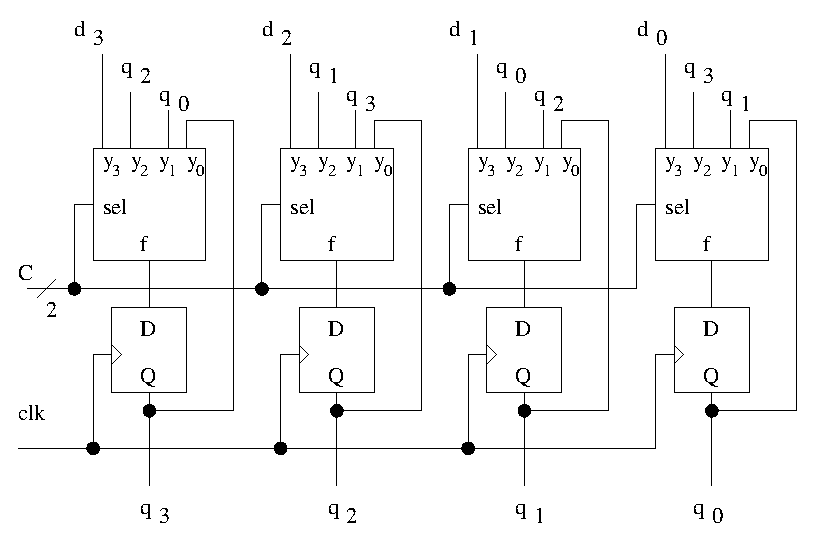
\includegraphics{./Fig6/ShiftReg}}
\caption{The internal organization of a 4-bit circular shift register.}
\label{fig:ShiftReg}

\end{figure}

The organization of the shift register is similar to the register, the 
difference being the larger mux.  When the 2-bit control signal,
denoted by the slash with a 2 through it, is 00, $Q_i$ is routed to
the input of each D flip flop.  The rising edge of the clock 
causes each D flip flop to latch its previous output, causing no 
change in the outputs.  When $C=01$, the data input to each D flip 
flop is $Q$, circularly shifted to the right.  This movement is denoted by
writing the name of each $Q$ bit on the mux input instead of drawing
the lines because otherwise the diagram quickly becomes messy and confusing.
Hence, when on the rising edge of the clock, the D flip flops 
latch the shifted value of the outputs, making all the outputs 
appear to circularly shift to the right, one bit.  The $C=10$ input
cause the inputs to circularly shift to the left.  The $C=11$ input,
sometimes called a parallel load because all four bits are loaded
simultaneously, loads each bit of the external 4-bit input, $D$, to its
respective flip flop.
\index{register!shift|)}

\section{The Counter}
A counter is a simple but surprisingly versatile piece of hardware.
Its behavior is obvious from its name; it counts up when instructed
to do so.

\index{counter|(}
\begin{tabular}{|l|p{3.5in}|} \hline

Nomenclature:  & N-bit counter with parallel load                  \\ \hline
Data Input:    & N-bits vector $D=d_{N-1} \ldots d_1 d_0$.          \\ \hline
Data Output:   & N-bit vector $Q=q_{N-1} \ldots q_1 q_0$    \\ \hline
Control:       & 2-bits $C=c_1 c_0$              \\ \hline
Status:        & none                                   \\ \hline
Others:        & 1-bit edge-sensitive clock.  1-bit asynchronous
                active low reset.                       \\ \hline
Behavior:      &

\begin{tabular}{c|c|c|c||c||c}

$reset$ & $clk$          & $C$  & $D$   & $Q^+$  & comment     \\ \hline
0     & x            & xx & x   & $0$    & reset       \\ \hline
1     & 0,1,falling  & xx & x   & $Q$    & hold        \\ \hline
1     & rising       & 00 & x   & $Q$    & hold        \\ \hline
1     & rising       & 01 & x   & $D$    & load        \\ \hline
1     & rising       & 10 & $D$   & $Q+1$  & count up    \\ \hline
1     & rising       & 11 & x   & x      &             \\

\end{tabular}	\\  \hline
\end{tabular}  
\label{page:counter}

When the 2-bit control input equals 10 and a clock edge arrives, the
counter counts up.  Since number of bits are limited, the 
counting will at some point overflow.  When this happens, the count
value rolls-over back to 0 and begins counting up again.
For example, a 4-bit counter rolls-over to 0 when it tries
to count up at 15.  This behavior is similar to the behavior of the digits of
a car's odometer rolling over from 9 to 0. 

A timing diagram for a 4-bit counter is shown in Figure~\ref{fig:CountTime}.
The initial value of the counter was arbitrarily set to $E_{16}=1110_2$.
At time=10, a positive edge of the clock arrives.  Since the $C$ input
is equal to $10_2$ at time=10, then the counter counts up to $F_{16}=1111_2$.
The goofy behavior of the $C$ input between time=10 and time=20 has
no effect on the $Q$ outputs of the counter because the clock is not rising.
At time=30, the $C$ input is equal to $00_2$ so the counter holds the current 
count value.  At time=50, the $C$ input is equal $10_2$ so the counter counts up
rolling over to $0_{16}$. At time=70 the counter counts up to $1_{16}=0001_2$.
At time=90, the counter loads $7_{16}=0111_2$.  Notice, as in 
Figure~\ref{fig:RegTime}, the counter timing diagram shows a small 
propagation delay for the $Q$ output.

\begin{figure}[ht]
\center{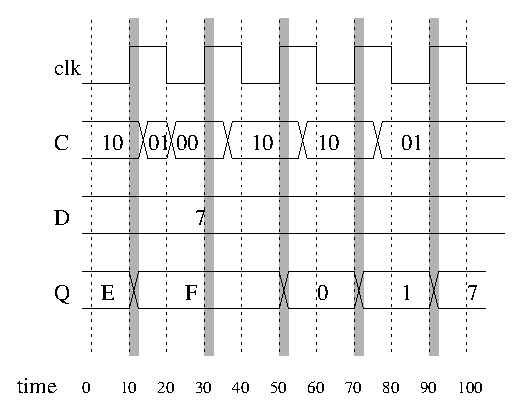
\includegraphics{./Fig6/CountTime}}
\caption{A timing diagram for a 4-bit counter.}
\label{fig:CountTime}
\end{figure}
\index{timing!counter}

The internal organization of a counter is very similar to the structure of
the register and shift register.  A set of D flip flops holds the current
count value.  A mux decides which input is presented to the D flip flops
to be latched up when the positive clock edge arrives.  An adder is
used to add 1 to the outputs of the flip flops (current count value).  
If the overflow output of the adder is ignored, then the adder has the 
advantage of rolling over to 0 when the count value is at the 
maximum.  It is easy to verify that 111...1 + 1 = 000...0.  The 
entire circuit is shown in Figure~\ref{fig:counter}.

\begin{figure}[ht]
\center{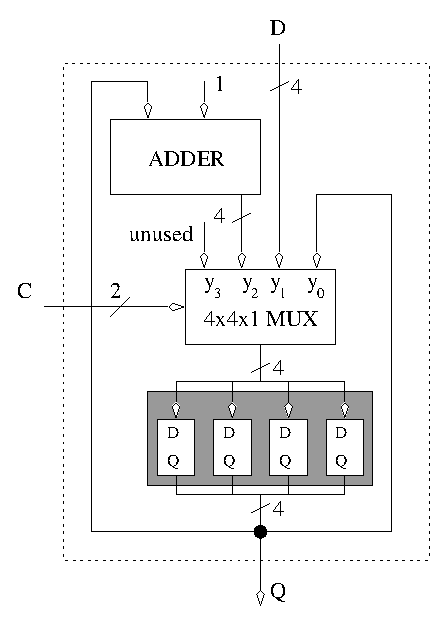
\includegraphics{./Fig6/counter}}
\caption{The internal organization of a 4-bit counter.}
\label{fig:counter}
\end{figure}

Notice, the data inputs to the mux shown in Figure~\ref{fig:counter}
all have a slash through them with
the number 4.  This notation indicates each of the data inputs is a four
bit wide
vector, and consequently, this device is a multibit mux, as discussed on 
page~\pageref{page:wmu}.  Additionally, the $y_3$ input is unused.  This
inefficiency is the cost of using a generalized building block.  
\index{counter|)}

\section{The Read Only Memory}
\pagebreak

\section{The Static RAM}
Random Access Memory (RAM) is an unfortunate name for a digital circuit 
that has nothing random about it.  The name ``RAM" originated in the early 
days of computing when engineers used cassette tapes as an inexpensive way 
to store ``lots" of data.  One of the downfalls of a cassette tape is the
sequential nature of data access.  That is, the time to access a piece of 
data depends on its position on the tape and the current position of the
tape.  RAMs are not sequential devices; the amount of time to access any
{\it random location} is the same.  

A wide variety of random access memories are available to meet the wide
variety of applications in which users need to store data.  For situations where
data needs to be retained even though power is removed, non-volatile memories are employed.  
The memories typically trade-off access and storage speed for the 
convenience of non-volatility.  Volatile memories, memories which lose
their contents when power is removed, can be either static/dynamic, or 
synchronous/asynchronous.  

Dynamic memories store data on tiny capacitors and
consequently require periodic refreshing in order to retain their values.  These versions
are typically the highest density memories available, but the refresh circuitry
adds to their complexity.  Static memories store data in an arrangement
of transistors which does not need refreshing.  Static memories generally 
consume much less power than their dynamic counterparts.  

Access to a synchronous memory requires a clock and is reminiscent of a flip flop.
Asynchronous memories require the control and data signals be applied
for certain minimum durations in order for the operations to take effect.

In order to convey the behavior and utilization of a RAM, consider one
of the most simple and utilitarian memories, the asynchronous static RAM.
The input, output, and behavior of asynchronous RAM is defined by the following table.

\index{RAM|(}

\begin{tabular}{|l|p{3.5in}|} \hline

Nomenclature:  & NxM RAM (random access memory)    \\ \hline
Data Input:    &  M-bit vector $D=d_{M-1} \ldots d_1 d_0$  
		$log_2(N)$-bit address $A=a_{log_2(N)-1} \ldots a_1 a_0$ \\ \hline
Data Output:   & M-bit vector $D=d_{M-1} \ldots d_1 d_0$	 \\ \hline
Control:       & 1-bit $CS$ (chip select), $R/W'$ (Read Write),        \\ \hline
Status:        & none                                   \\ \hline
Others:        & none                 \\ \hline
Behavior:      &
			\begin{tabular}{c|c|c||c|l}
			$A$ & $CS$  & $R/W'$ & $D$  	& Note   	       \\ \hline
			x   & 0     & x      & $Z$  	& RAM deactivated      \\ \hline
			$A$ & 1     & 0      & $D$  	& RAM[$A$] = $D$ (write) \\ \hline
			$A$ & 1     & 1      & RAM[$A$]	& $D$ = RAM[$A$] (read)  \\
			\end{tabular} \\ \hline

\end{tabular}
\label{page:ram}

A RAM is a storage device that stores and retrieves bundles of bits, called 
a word, stored at an address.  Envision a RAM as an array
of binary numbers.  The width of a RAM is called
the word size.  Each word in the RAM has an address. By convention addressing
starts at Location 0. The following process is used in order to read data out 
of a RAM:

\begin{tabular}{l}

1. Assert the address $A$, $CS$ and $R/W'=1$ \\
2. Wait \\
3. Read $data$ \\

\end{tabular}

Assume the contents of the RAM are shown in Figure~\ref{fig:ram}.
If $A=101_2=5_{10}$ and $CS=R/W'=1$ then a little while later $D=0001$.  

\begin{figure}[ht]

\center{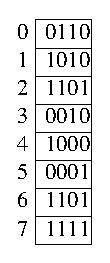
\includegraphics{./Fig6/ram}}
\caption{A 8x4 RAM has eight words each containing four bits.  The addresses
(which are not stored in the RAM) are shown to the left.}
\label{fig:ram}

\end{figure}

The notation \verb^ D = RAM[A]^ used to describe the read operation
in the RAM's truth table is reminiscent of array access in a 
typical programming language.  Notice, the data 
$D$ is used as both input and output.  Hence, a RAM can either read 
or write over the same set of lines, but not both at the same time. 
Writing data into a RAM is a 3-step process:

\begin{tabular}{l}

1. Assert $data$ and the address $A$. \\
2. Assert $CS$ and $R/W'=0$ \\
3. Wait \\

\end{tabular}

Consider the contents of the RAM shown in Figure~\ref{fig:ram}.
If $A=110_2=6_{10}$, $CS=1$, $R/W'=0$, and $D=0101$, then a little while 
later the memory word at address 6 would be changed from $1101$ to
$0101$.  

While there is no relationship between the word size and the number of 
words stored in the RAM, there is a relationship between the number
of words stored in the RAM and the number of address bits:
The number of bits in the address must be sufficient to assign 
each word a unique binary address.  The $N$ address bits can be arranged 
in $2^N$ different ways.  Hence, a RAM with $N$ address lines can have 
up to $2^N$ words.  The number of words in a RAM is often described 
using the metric system notation.

\begin{tabular}{ccc}

1k & $2^{10}$ & kilo \\ 
1M & $2^{20}$ & mega \\ 
1G & $2^{30}$ & giga \\ 
1T & $2^{40}$ & tera \\ 

\end{tabular}

The metric names are only close approximations to the actual, binary values
they describe.  For example, 1 kilometer is a 1,000 meters, but 
1k bytes of memory is $2^{10}$ bytes, or $1024$ bytes.  The number of 
address bits can be determined quickly from the metric abbreviations.
For example, a 256k RAM has $256k=2^8*2^{10}=2^{18}$ words, or 18 bits 
of address.

Cases occur when it is necessary to build a larger RAM from several
smaller RAMs.  RAMs have two dimensions which can be increased: (1) the word size or 
(2) the number of words.  

Increasing the word size of a RAM is fairly straightforward because 
each RAM chip gets all the address lines and handles some portion of 
the data lines.  Structurally, this transformation is accomplished by
placing several RAM chips side-by-side as shown. For example, in order 
to construct a 256kx32 RAM from 256kx8 RAM chips, then four, 256kx8 RAM are 
placed side-by-side as shown in Figure~\ref{fig:ram}.

\begin{figure}[ht]
\center{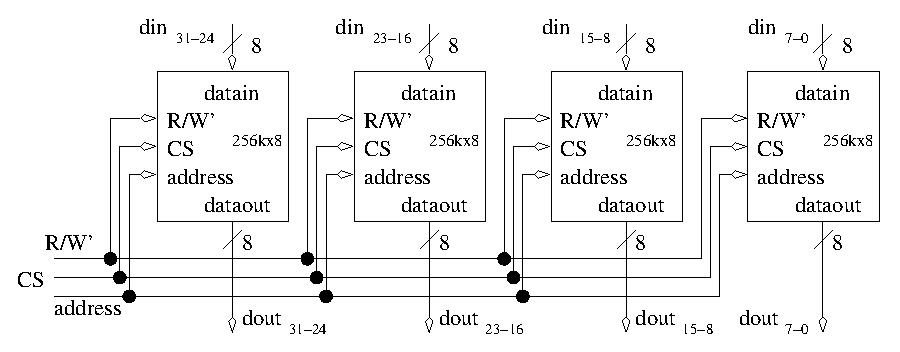
\includegraphics{./Fig6/wide}}
\caption{The construction of a 256kx32 RAM from 256kx8 RAM chips.}
\label{fig:wide}
\end{figure}

Each of the four chips have the same address lines and control
lines $R/W'$, and $CS$.  Thus, all the RAM chips behave in exactly the same 
fashion, each handling its own set of eight bits.  Their actions are coordinated
by the common address and control signals.

Combining RAM chips to increase the number of words involves some manipulation
of addresses.  For example, consider the problem of using 64kx8 RAM chips to 
construct a circuit which behaves like a 256kx8 RAM.  Stacking four, 64kx8 RAM
chips above one another would create the required depth of 256k words.  However,
each of the 64k RAMs would have 16 address lines, but the 256k RAM being 
constructed requires 18 address lines.  How is this discrepancy of the extra 
two address bits resolved?  The 18 bits of address are split into two 
components; the lower 16 bits are sent to all four of the 64kx8 RAMs 
and the upper two bits are used to decide which of the four 64k RAM chips 
is activated.  A decoder uses
the two bits as select, and routes a chip select signal to one of its four outputs
which are attached to the chip select lines of each 64k RAM.  Since a decoder
routes the chip select to only one of the RAMs, there is no potential 
conflicts on the data lines and they can safely be tied together. 
Figure~\ref{fig:deep} shows the complete circuit diagram.

\begin{figure}[ht]

\center{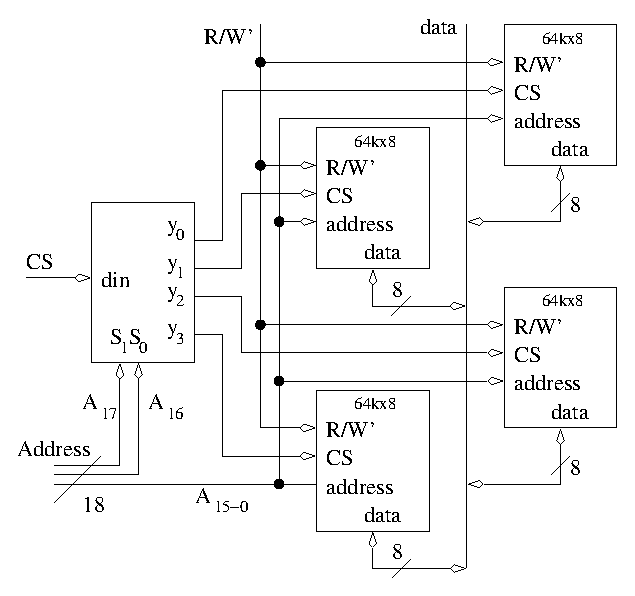
\includegraphics{./Fig6/deep}}
\caption{The construction of a 256kx4 RAM from 64kx4 RAM chips.}
\label{fig:deep}

\end{figure}
\index{RAM|)}

\section{The Dynamic RAM}
\pagebreak

\section{Register Transfer}
A digital system designed using the datapath and control approach 
transforms data into some predetermined sequence.  For now, focus 
on the task of transforming the data performed by the datapath.  
The datapath is composed of the basic building blocks discussed in 
Chapters 4 and 6; their input, output and behavior is summarized on 
page~\pageref{page:boxlist}.  Although a gross simplification, a 
datapath can be considered as some combinational logic ``sandwiched" 
between registers.  The clock signal to the datapath governs how 
data moves in the datapath. After the rising edge of the clock, the 
register outputs become valid. The output data from the registers 
flows into the combinational logic which transforms this input into 
an output.  The outputs of the combinational logic flow into the 
register inputs.  The next rising edge of the clock causes the 
registers to latch these new values.  This process then proceeds 
into the next clock cycle.  In order to understand this discussion, 
consider the simplified datapath shown in Figure~\ref{fig:simple}.  
In this datapath, an adder is sandwiched between three registers.  
Here, the control inputs on all three registers are assumed to be 
hardwired to 1, causing them to load on every positive edge.  The 
inputs $A$ and $B$ to the two registers are provided by some 
external agent.
  
\begin{figure}[ht]

\center{\scalebox{0.8}{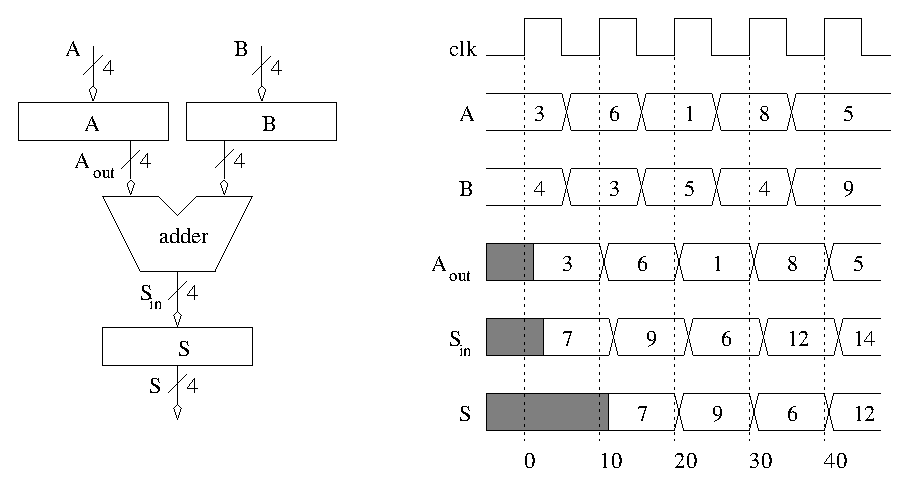
\includegraphics{./Fig6/simple}}}
\caption{A simple datapath and the timing diagram describing its
behavior.}
\label{fig:simple}

\end{figure}

When a signal has an unknown value, it is given a shaded regions.  Prior to 
time=0, none of the registers contains a known value, therefore all 
their outputs are shaded.  Since $A=3$ and $B=4$ prior to the 
positive edge at time=0, the outputs of register $A/B$ equals 3/4 
after the positive edge at time=0, respectively. The slight delay 
in the $A_{out}$ signal becoming valid, emphasizes how the 
real outputs of a register exhibit propagation delay. Note, the output of the
$B$ register is not shown because its behavior is similar to $A_{out}$ and
would clutter up the timing diagram.  Since the outputs of the $A$ and $B$ 
registers are unknown prior to time=0, causing the 
inputs to the adders to be unknown, causing the outputs of the 
adder to be unknown, causing the input to the $S$ register to be 
unknown.  Since the inputs to the $S$ 
register are unknown when the clock edge arrives at time=0, the outputs of the
$S$ register remain unknown after that clock edge.  

It might seem as if the new outputs of registers $A/B$ available 
just after the clock edge at time=0 would be able to propagate 
to the $S$-register's input, allowing it to latch a valid value 
on the time=0 clock edge.  This is incorrect because all the
registers in the datapath latch their values at exactly the same 
instant in time and then output their new values.  This assertion 
is simply a restatement of the observation made on 
page~\pageref{page:FFdelay}: the propagation delay of a flip flop 
should be larger than the hold time in order to allow flip flops 
to be daisy-chained together.

The $A$ and $B$ signals are changed at time=5, on a negative edge 
of the clock, in order to keep the changes on the register inputs 
as far away from a positive edge of the clock as possible.

After the rising edge of the clock at time=0, the outputs of the 
$A$ and $B$ registers become valid, causing the inputs to the adder 
to become valid, causing the output to become valid, causing the 
input to the $S$ register to become valid.  Thus, the $S_{in}$ 
signal becomes valid after the positive clock edge at time=0.

When the positive clock edge at time=10 arrives at the circuit in 
Figure~\ref{fig:simple}, registers $A/B/S$ latch the values on their 
inputs, 6/3/7, respectively.  The new outputs of $A$ and $B$ are 
sent to the adder causing $S_{in} = 9$.  This value cannot be 
latched into the $S$ register until the next rising edge of the 
clock at time=20, because the rising edge at time=10 is long gone.

The positive clock edge at time=20 causes registers $A/B/S$ to latch 1/5/9, 
respectively.  Once the analysis is started, it is a matter of waiting for a 
positive clock edge, latch all the register inputs simultaneously, propagating 
outputs through the combinational logic, and waiting for the next positive edge.
                                                                                

%%------------------------------------------------
%% Add a complex analysis problem here that uses
%% the reset and control lines.
%%------------------------------------------------

\section{Combinations}
The basic building blocks in Chapters 4 and 6 can be combined in interesting ways
to produce complex behavior.  The behavior of these digital systems can be described 
using a programming-language-like syntax, initially presented in Chapter 4. First, examine
the counter, counting over a subinterval of its possible range.

\begin{verbatim}
    while(1) {
        if (count<10) count += 1;
        else count = 3;
    }
\end{verbatim}

The \verb+while(1)+ statement means that the statements contained 
in \verb+while+-brackets should be executed forever.  In other 
words, it is a never-ending loop.  The \verb+if+ statement checks 
the count value. If it is less than 10, \verb+count+ is incremented, 
otherwise the value is reset back to 3. The circuit is implemented 
with a counter to perform the count-up function and a comparator 
to perform the magnitude comparison between \verb+count+ and 9.  
Why 9?  Because if the value is compared against 10, then the 
\verb+count+ value would have to reach 10 in order for the $L$ 
output of the comparator to change, by which time it would be too 
late to stop the \verb+count+ value from reaching 10.  The completed 
circuit and a timing diagram is shown in Figure~\ref{fig:comb1}.

\begin{figure}[ht]
\center{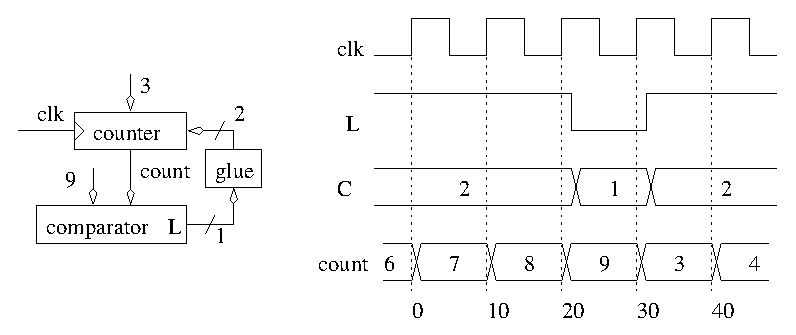
\includegraphics{./Fig6/comb1}}
\caption{A circuit to count between 3 and 9 and its associated timing diagram.}
\label{fig:comb1}

\end{figure}

The $L$ output of the comparator is used because the condition checked is 
\verb+count < 10+.  This single-bit output cannot be directly connected to the
counter's 2-bit control input because there just are not enough bits.  The
``glue" box shown in Figure~\ref{fig:comb1} contains glue-logic, a
combinational logic circuit which interfaces or glues together two pieces
of logic.  When the counter's output is less than 10, $L=1$, and the
counter is supposed to count up by 1.  According to 
page~\pageref{page:counter}, this requires the control to be $c_1c_0=10$.

When the counter's output is greater than or equal to than 10, $L=0$, 
the counter should load 3.  According to 
page~\pageref{page:counter}, a load is elicited by asserting 
$c_1c_0=01$ on the counter's control input.  The 
resulting truth table for the glue logic is shown in the margins.  
From this table, it is easy to ascertain that $c_1 = L$ and $c_0 = L'$.

\marginpar { \tiny
$$\begin{array}{c||c|c}
L & c_1 & c_0	\\ \hline \hline
0 & 0 & 1 		\\ \hline
1 & 1 & 0 		\\ 
\end{array} $$
}

The timing diagram shows the counter starting at 6.  Since 6 is less 
than 10, then $L=1$.  When $L=1$ is present on the input of the
glue logic it will output $C=c_1c_0=10$, causing the counter
to count up when the clock input arrives at time=0.  Successive clock edges
see the count value increment to 9 at time=20.  At this moment, the $L$ output
of the comparator changes to 0 causing the glue logic box to output 
$C=c_1c_0=01$ telling the counter to load 3 on the next positive clock edge 
at time=30.  When the value of 3 is loaded into the counter at time=30, the
$L$ output of the comparator changes to 1, causing the glue logic box to
tell the counter to count up on the next positive clock edge at time=40.
Without a finite state machine, it is difficult to get a combination of basic 
building blocks to perform a sequence of actions. Difficult, but not 
impossible as the following circuit shows.
 
Design a circuit which searches the first 
100 memory locations of an eight bit wide random access memory for the smallest 
value is examined.  Assume the RAM is preloaded with data values, so 
only the memory needs to be read.  The approach reads each value 
and checks if it is smaller than the smallest 8-bit value found
thus far.  This smallest value is stored in a register, \verb+min+, which
will be assumed as initialized to the largest possible value, 0xFF.  The ``0x"
in front of ``0xFF" is used in many program languages to signify that 
``FF" is a hexadecimal number.
\label{page:minsearch} 

\begin{verbatim}
    // assume that min is initialized to 0xFF
    for(i=0; i<100; i++) {
        MBR = RAM[i];
        if (MBR < min) MBR = min;
    }
\end{verbatim}

The variable \verb+MBR+, standing for memory buffer register, is a generic
term applied to a register used to buffer data operations between a RAM and 
a datapath.  The line \\
\verb^for(i=0; i<100; i++)^ will be implemented with a 
counter and a comparator.  The comparator examines the counter's output and  
stops the counter when the count value reaches 99.  The line 
\verb+MBR = RAM[i];+ is implemented with a RAM and a register.  The address
of the RAM \verb+[i]+ comes from the counter, and the data output of the RAM
is sent to the data input of a register called MBR.  The line 
\verb+if (MBR < min) MBR = min;+ is realized with a comparator and 
a register.  The comparator compares the output of the MBR and the min
registers and asserts its $L$ output when MBR is less than min.  This 
$L$ output runs to the control input of the min register.  The data 
input of the min register comes from the data output of the MBR 
register.  The control of the MBR register should also be controlled 
by the counter comparator so that the MBR register stops loading when 
the count value is greater or equal to 99.  The circuit diagram is 
shown in Figure~\ref{fig:min} 

\begin{figure}[ht]
\center{\scalebox{0.8}{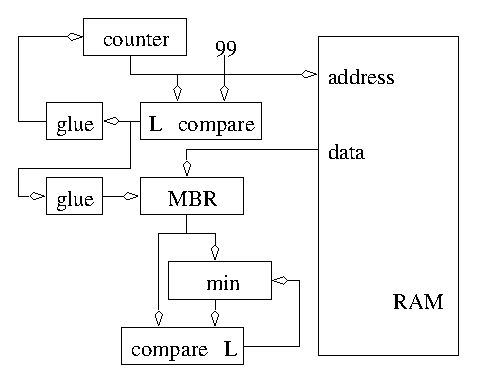
\includegraphics{./Fig6/min}}}
\caption{A circuit to find the smallest value in a RAM.  The min 
register is initialized to 0xFF.}
\label{fig:min}
\end{figure}

\section{Timing}
\pagebreak
.
\pagebreak
.
\pagebreak
.
\pagebreak
.
\pagebreak
.

\section{Exercises}
\section{Exercises}
\label{section:sequentialBB}
\graphicspath{ {./chapter06/FigHw} }

\begin{enumerate}
    \item \textbf{ (8 points)} Build a 4-bit universal shift register in
        Table~\ref{table:uni} using D flip-flops and 8:1 multiplexers.

        \begin{table}
            \begin{tabular}{c|c|c||c}
                S2 & S1 & S0 & Operation \\ \hline
                0  &  0 &  0 & Hold \\ \hline
                0  &  0 &  1 & Load \\ \hline
                0  &  1 &  0 & ASR  \\ \hline
                0  &  1 &  1 & ASL  \\ \hline
                1  &  0 &  0 & LSR  \\ \hline
                1  &  0 &  1 & LSL  \\ \hline
                1  &  1 &  0 & CSR  \\ \hline
                1  &  1 &  1 & CSL  \\
            \end{tabular}
            \caption{The truth table for a universal shift register.}
            \label{table:uni}
        \end{table}

        \begin{onlysolution}  \textbf{Solution} \itshape{
                \begin{figure}[ht]
                    \center{
\includegraphics{Prob6-1}}
                \end{figure}
            }
        \end{onlysolution}

    \item \textbf{ (8 pts.)} Use a counter and a comparator
        to implement the following circuits.

        \begin{enumerate}
            \item Show how to modify the counter (by adding some external logic)
                to implement a mod-10 counter.  A mod-10 counter counts from 0 to
                9 and then goes back to 0.  It spends one full clock cycle on each
                of these count values.

                \begin{onlysolution}  \textbf{Solution} \itshape{
                        Our mod 10 counter will have 1 data input, representing
                        the state of the least significant counter.  Call this input
                        Nine In.  Nine In equals 1 when the less significant counters
                        output equals 9, otherwise Nine In equals 0.  Our mod 10 counter
                        will have four bits of output representing the current count value.
                        The mod 10 counter will also have a Nine Out output which will
                        equal 1 when our current count value equals 9, otherwise
                        Nine Out equals 0.  Let the constant value 9 be sent to the Y
                        input of the comparator and the 4-bit register (Q) sent to the X
                        input.  When Q<9 the comparator outputs G=0, L=1, E=0.  When
                        Q=0 then the comparator outputs G=0, L=0, E=1.  Hence by running
                        the E output of the comparator to the select input of the mux,
                        the Q+1 will be sent to the register input when Q<9.  Notice
                        that the register will only latch a new value (Q+1 or 0) when
                        the less significant counter has rolled over.

                        \begin{figure}[ht]
                            \center{
\includegraphics{Prob6-2}}
                        \end{figure}

                    }
                \end{onlysolution}

            \item Use four mod-10 counters to build a 4-digit decimal counter which
                counts up from 0 to 9999.  Draw a schematic for the 4-digit decimal
                counter.

                \begin{onlysolution}  \textbf{Solution} \itshape{
                        Just ripple four of the above counter head to tail via Nine In and Nine
                        Out.  Set the Nine In input of the least significant counter to 1.
                    }
                \end{onlysolution}

        \end{enumerate}

    \item \textbf{ (8 pts.)} Design a circuit which contains three 8-bit
        registers X,Y,Z.  The behavior of the circuit is determined by the statement:
\begin{verbatim}
if (X > Y) then Z = X+X else Z = Y+Y
\end{verbatim}
        The registers are preloaded with values in them.
        Submit a circuit diagram showing the building blocks uses,
        their interconnections and any miscellaneous logic required to make
        them operate together.
        \begin{onlysolution}  \textbf{Solution} \itshape{
                \begin{figure}[ht]
                    \center{
\includegraphics{Prob6-3}}
                \end{figure}
            }
        \end{onlysolution}

    \item \textbf{ (8 pts.)} Design a circuit which contains three registers X,Y,Z.
        The behavior of the circuit is determined by the statements:
\begin{verbatim}
1. while (X > 0) {
2.     Z = Z+Y;
3.     X = X-1;
4. }
\end{verbatim}
        The registers are preloaded with values in them.
        Submit a circuit diagram showing the building blocks used,
        their interconnections and any miscellaneous logic required to make
        them operate together.  The design should use an adder and an
        adder subtractor plus some other building blocks.  Hint, use
        the enable inputs of the registers to control when they
        latch information.

        \begin{onlysolution}  \textbf{Solution} \itshape{
                \begin{figure}[ht]
                    \center{
\includegraphics{Prob6-4}}
                \end{figure}
            }
        \end{onlysolution}

    \item \textbf{ (8 pts.)} Given three 32-bit registers A,B,PC, design a circuit
        which adds PC and A (putting the result back into PC) when A is equal
        to B.  Otherwise, add 1 to PC.  The contents of A and B
        are to remain unchanged.

        \begin{onlysolution}  \textbf{Solution} \itshape{
                \begin{figure}[ht]
                    \center{
\includegraphics{Prob6-5}}
                \end{figure}
            }
        \end{onlysolution}

    \item \textbf{ (8 pts.)} Build a circuit that performs the following:
\begin{verbatim}
    for(i=0; i<100; i++)
        total = total + i;
\end{verbatim}
        Use the counter described in this chapter for the $i$ variable;
        assume that the counter is initialized to 0. \verb^total^ is stored
        in a register and its initialized to 0.  Use a comparator to shut
        down the counter and put the register in hold when the count value
        reaches a critical value. Until this critical value is
        reached the comparator should allow the counter to count and the
        register to load.

        \begin{onlysolution}  \textbf{Solution} \itshape{
                Note that the counter really needs only one of two control settings
                00 for holding and 10 for counting up.  Thus, the LSB of the counters
                control input can be hardwired to 0.  Its the MSB of the counters control
                that needs controlled by the comparator.  Since the counter is in the
                range of 0-100, the counter has a 7-bit output.  It is an interesting exercise to
                determine the number of bits required for the adder's output so that it
                does not overflow during the computation.  The figure below shows that
                13 bits are required (the upper six bits of the counter's output are padded
                with 0's so that the counters output can be feed into the adder).

                \begin{figure}[ht]
                    \center{
\includegraphics{Prob6-6}}
                \end{figure}
            }
        \end{onlysolution}

    \item\textbf{ (8 pts.)} Build a circuit that performs the following:
\begin{verbatim}
    for(i=0; i<100; i++)
        total = total + 1;
\end{verbatim}

        \begin{onlysolution}  \textbf{Solution} \itshape{
                \begin{figure}[ht]
                    \center{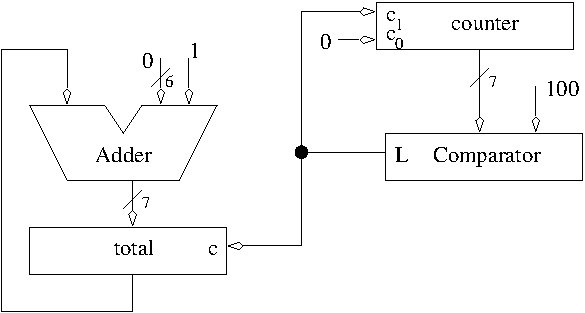
\includegraphics{Prob6-7}}
                \end{figure}
            }
        \end{onlysolution}

    \item\textbf{ (8 pts.)} Design a circuit that can shift (circular
        to the right) the contents of register X by an amount given in
        register Y. X is stored in the circular shift register described
        in this chapter. The solution will require a comparator and a
        counter.
        \begin{onlysolution}  \textbf{Solution} \itshape{
                \begin{figure}[ht]
                    \center{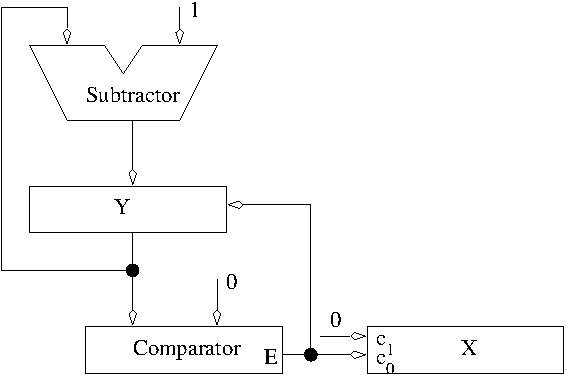
\includegraphics{Prob6-8}}
                \end{figure}
            }
        \end{onlysolution}

    \item\textbf{ (8 pts.)} Assume a 32kx8 RAM is full of data. Show
        the hardware required to realize the following algorithm.
\begin{verbatim}
    for(i=0; i<32767; i++)
        total = total + M[i];
\end{verbatim}

        Where \verb+M[i]+ is the 8-bit word stored at address \verb^i^.
        Assume the total register is initialized to 0. The $i$ variable should
        be the output of a counter. Use a comparator to shut down the counter
        and to put the register in hold when the count value reaches a critical
        value.
        \begin{onlysolution}  \textbf{Solution} \itshape{
                \begin{figure}[ht]
                    \center{
\includegraphics{Prob6-9}}
                \end{figure}
            }
        \end{onlysolution}

    \item\textbf{ (8 pts.)} Show how to initialize a 32kx8 RAM in the following manner.
\begin{verbatim}
    for(i=0; i<32767; i++)
        M[i] = i mod 256;
\end{verbatim}

        Where the ``i mod 256" statement means store the least significant
        eight bits of the $i$ variable into the RAM.

        \begin{onlysolution}  \textbf{Solution} \itshape{
                \begin{figure}[ht]
                    \center{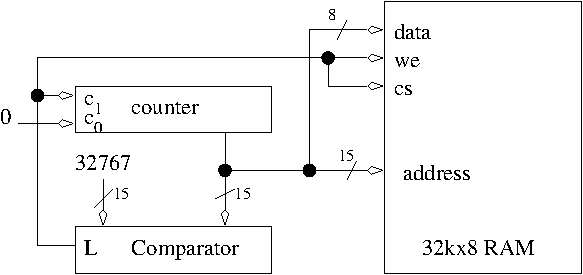
\includegraphics{Prob6-10}}
                \end{figure}
            }
        \end{onlysolution}

    \item\textbf{ (5 pts.)} Complete the timing diagram in Figure~\ref{fig:hwshift}
        \label{item:shifter}
        for a 4-bit arithmetic shift register.  Use the control setting from the
        truth table on page~\pageref{page:shi}.
        \begin{figure}[ht]
            \center{
\includegraphics{Prob6-14}}
            \caption{The timing diagram for a 4-bit arithmetic shift register in
            Problem~\ref{item:shifter}.}
            \label{fig:hwshift}
        \end{figure}

        \begin{onlysolution}  \textbf{Solution} \itshape{
                \begin{figure}[ht]
                    \center{
\includegraphics{Prob6-13}}
                \end{figure}
            }
        \end{onlysolution}

    \item\textbf{ (5 pts.)} Complete the timing diagram in Figure~\ref{fig:hwcount}
        \label{item:counter}
        for a 4-bit counter.  Use the control setting from the truth table on
        page~\pageref{page:counter}.
        \begin{figure}[ht]
            \center{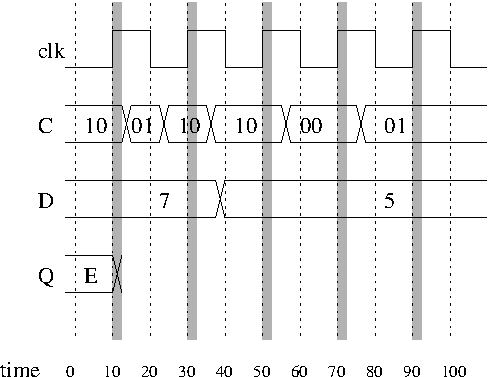
\includegraphics{Prob6-15}}
            \caption{The timing diagram for a 4-bit counter in
            Problem~\ref{item:counter}.}
            \label{fig:hwcount}
        \end{figure}

        \begin{onlysolution}  \textbf{Solution} \itshape{
                \begin{figure}[ht]
                    \center{
\includegraphics{Prob6-14}}
                \end{figure}
            }
        \end{onlysolution}

    \item\textbf{ (5 pts.)} Complete the timing waveforms for $A_1, A_0, Q_1, Q_0$
        \label{item:cascade}
        based on the circuit diagram shown in Figure~\ref{fig:cascade}.  Use the truth
        table on page~\pageref{page:reg} for the register. Put the decimal
        representation of the signals in the timing diagram (like the timing
        diagram in Figure~\ref{fig:comb1}).
        \begin{figure}[ht]
            \center{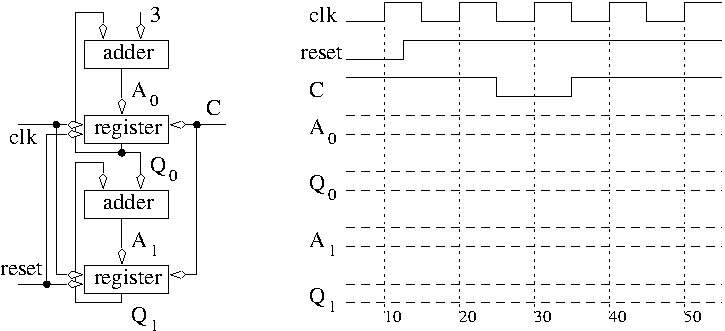
\includegraphics{Prob6-16}}
            \caption{The circuit diagram and incomplete timing diagram for
            Problem~\ref{item:cascade}.}
            \label{fig:cascade}
        \end{figure}

        \begin{onlysolution}  \textbf{Solution} \itshape{
                \begin{figure}[ht]
                    \center{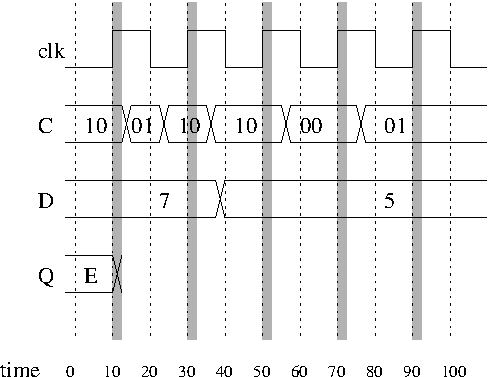
\includegraphics{Prob6-15}}
                \end{figure}
            }
        \end{onlysolution}

    \item\textbf{ (4 pts.)} The circuit shown in Figure~\ref{fig:fib} generates a
        Fibonacci sequence, a sequence starting with 1,1,2,3...  The next number in
        the sequence is the sum of the preceding two numbers.  Complete the
        timing diagram, assuming the circuit starts with the values shown.
        Identify the signal which generates a complete Fibonacci sequence.

        \begin{figure}[ht]
            \center{
\includegraphics{fib}}
            \caption{A circuit which generates a Fibonacci sequence.}
            \label{fig:fib}
        \end{figure}

\end{enumerate}


